\documentclass{article}

\usepackage{fancyhdr} % Required for custom headers
\usepackage[utf8]{inputenc}
\usepackage{lastpage} % Required to determine the last page for the footer
\usepackage{extramarks} % Required for headers and footers
\usepackage[usenames,dvipsnames]{color} % Required for custom colors
\usepackage{graphicx} % Required to insert images
\usepackage{listings} % Required for insertion of code
\usepackage{color}
\usepackage{courier} % Required for the courier font
\usepackage{lipsum} % Used for inserting dummy 'Lorem ipsum' text into the template
\usepackage[norsk]{babel}
\usepackage{amsmath}

% Margins
\topmargin=-0.45in
\evensidemargin=0in
\oddsidemargin=0in
\textwidth=6.5in
\textheight=9.0in
\headsep=0.25in

\linespread{1.1} % Line spacing

% Set up the header and footer
\pagestyle{fancy}

\lhead{\exerciseGroup} % Top left header
\chead{\exerciseClass: \exerciseTitle} % Top center head
\rhead{\firstxmark} % Top right header
\lfoot{\lastxmark} % Bottom left footer
\cfoot{} % Bottom center footer
\rfoot{Page\ \thepage\ of\ \protect\pageref{LastPage}} % Bottom right footer
\renewcommand\headrulewidth{0.4pt} % Size of the header rule
\renewcommand\footrulewidth{0.4pt} % Size of the footer rule

\setlength\parindent{0pt} % Removes all indentation from paragraphs


% Document data

\newcommand{\exerciseTitle}{Øving 6} % Assignment title
\newcommand{\exerciseClass}{TMA4280} % Course/class
\newcommand{\exerciseGroupMembers}{Sindre Magnussen og Håkon Åmdal}
%----------------------------------------------------------------------------------------
%	TITLE PAGE
%----------------------------------------------------------------------------------------
\newcommand{\HRule}{\rule{\linewidth}{0.5mm}}
\title{
\vspace*{\stretch{1}}
\noindent\HRule
\begin{center}
 \Huge
 \noindent	\exerciseClass \\
 \noindent \exerciseTitle \\ [4mm]
 \large
 \noindent\emph{\exerciseGroupMembers}
\noindent\HRule \newline
\end{center}
\vspace{0cm}
\begin{center}
	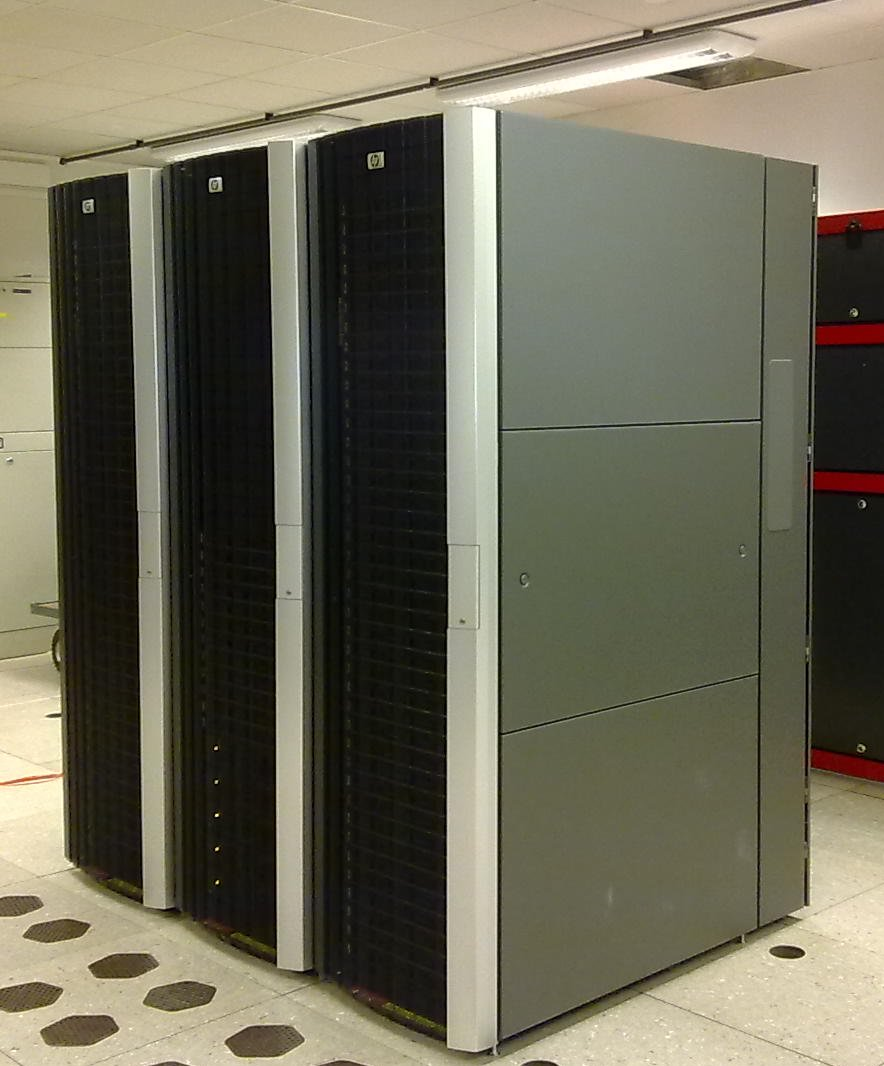
\includegraphics[width=10cm]{img/kongull.jpg}
\end{center}
\vspace*{\stretch{3}}
\begin{center}
\end{center}
}
% Insert date here if you want it to appear below your name

\newcommand{\ub}[1]{\underbar{$#1$}\,}
\definecolor{mygreen}{rgb}{0,0.6,0}
\definecolor{mygray}{rgb}{0.5,0.5,0.5}
\definecolor{mymauve}{rgb}{0.58,0,0.82}
\lstdefinestyle{customc}{
  belowcaptionskip=1\baselineskip,
  breaklines=true,
  frame=L,
  xleftmargin=\parindent,
  language=C,
  showstringspaces=false,
  basicstyle=\footnotesize\ttfamily,
  keywordstyle=\bfseries\color{green!40!black},
  commentstyle=\itshape\color{purple!40!black},
  identifierstyle=\color{blue},
  stringstyle=\color{orange},
}
\lstset{escapechar=@,style=customc}


\begin{document}
\pagestyle{empty}
\maketitle

\thispagestyle{empty}

\newpage \tableofcontents


\newpage

\pagenumbering{arabic}

\section{Introduksjon - Poisson-problemet}
Poisson-ligningen er en av de mest kjente partielle diffensialligingene, og skrives på formen:
\begin{equation}
	-\nabla^2 u = f
\end{equation}
Her er $\nabla^2$ kjent som Laplace-operatoren.\\
\\
Liginingen brukes som en matematisk modell til å beskrive flere fysiske systemer, som oftest diffusjonsprosesser. Eksempler på typiske fysiske fenomener hvor poisson-ligningen kan brukes som modell er beregning av elektrisk felt, tilnærminger av strømninger i fluider og varmeoverføring uten varmetap. Poisson-ligingen dukker også opp når man skal regne ut egenverdier.\\
\\
Et poissonproblem er et problem der man skal finne en løsning til poisson-ligningen gitt en funksjon $f$ og et domene. Domenet har også grensebetingelser, slik at problemet har en unik løsning. Problemet vi skal løse i denne øvingen lyder som følgende:
% Dette er tatt direkte fra ps6.tex %
\begin{eqnarray}
	-\nabla^2 u & = & f \hspace{.5in} \textrm{in} \,\,\, \Omega = (0,1)\times (0,1) \\
	u & = & 0 \hspace{.5in} \textrm{on} \,\,\, \partial\Omega\, .
\end{eqnarray}
Her er $f$ en funksjon vi kjenner,  og $u$ er løsningen vi skal komme frem til. Vi har gitt at et enhetskvadrat  er vårt domenee, og at verdiene i kantene av dette kvadratet er $0$ (homogene Dirichlet grensebetingelser). Vi kan ikke gjøre noen antagelser om $f$, annet at den er reell.
\emph{AM - Er den reell?}\\
\\
Siden denne skal løses på en datamaskin, og en datamaskin har begrenset med ressurser (minne/regnekraft), må vi finne en tilnærming til løsningen $u$. Det finnes flere måter å diskretisere poisson-ligningen på (finite differences, finite elements and finite volumes \emph{AM - Hva heter dette på norsk?}), men alle disse ender opp med et sett med ligninger som kan skrives på formen:
\begin{equation}
	\label{eq:linear-system}
  \ub{A} \ub{u} = \ub{g}
\end{equation}

\begin{figure}[t]
	\label{fig:finite-difference}
	\centering
	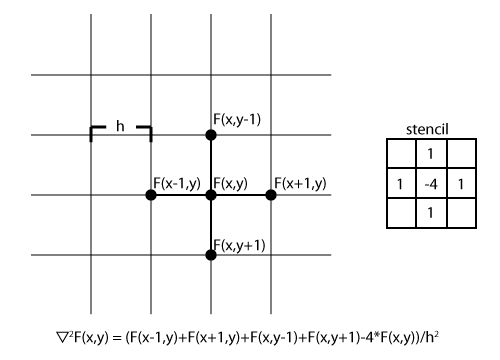
\includegraphics[width=10cm]{img/finite-difference.png}	
	\caption{Oppretting av et ligningsystem ved hjelp av endelige differanser. Figur funnet på \cite{rdw}. }
	
\end{figure}

Siden \emph{TMA4280} underviser i endelige differanser, og dette er ofte beskrevet som den enkleste metoden, er dette også utgangspunktet for denne oppgaven. Oppgaven beskriver et todimensjonalt poissonproblem, og da fylles ligningssettet ut med en maske som vist i figur \ref{fig:finite-difference} (fempunktsformelen).

\section{Mulige løsningsstragegier}
Når vi har fått et ligningssystem på formen vist i ligning \ref{eq:linear-system}, gjenstår det å finne en metode å løse dette på. Det finnes mange metoder, og noen av metodene utnytter egenskaper ved ligningssystemene fra poissonproblemet for å effektivisere plassforbruk og kjøretid.
\subsection{Direkte metoder}
Dirkete metoder løser et system med ligninger i et endelig og forutsigbart antall steg, og er spesielt egnet når matrisene er symmetriske og positivt definitt (som ligningssettet produsert ved hjelp av endelige differanser). Eksempelet på den mest generiske direkte metoden er LU-faktorisering, med følgende asymptotiske egenskaper:
\begin{align*}
      \mathcal{N}_{op} &\sim \mathcal{O}(N^3), \\
      \mathcal{M} &\sim \mathcal{O}(N^2).
\end{align*}
Her er $N$ antall ukjente,  $\mathcal{N}_{op}$ antall FLOP og $\mathcal{M}$ minnebruk (i bytes). Flere optimaliseringer av LU-faktoriseringer finnes, det er særlig vanlig å utnytte at matrisen er \emph{AM - sparse} for å redusere minnebruk og antall flyttallsoperasjoner. \\
\\
Ved å utnytte ligningen som blir generert av fem-punktsformelen, kan vi diagonalisere ligningssystemet ved hjelp av egenvektorer og egenverdier. Egenskaper ved det to-dimensjonale poissonproblemet gjør at vi kan utnytte at ligningssytemet vårt kan representeres ved et tensorprodukt, og dette forenkler utregningen av egenvektorer og egenverdier.\\
\\
En av disse diagonaliseringsmetodene benytter seg av FFT (The Fast Fourier Transform), og har følgende asymptotiske egenskaper:
\begin{align*}
  \mathcal{N}_{op} &\sim \mathcal{O}(N \log N), \\
  \mathcal{M} &\sim \mathcal{O}(N).
\end{align*}
Denne tilnærmet optimale løsningen er strategien vi skal bruke for å løse poisson-problemet i denne øvingen.
\emph{AM - Hvorfor er denne optimal?}

\subsection{Iterative metoder}
I tillegg til direkte metoder, har vi også iterative metoder. En slik metode vil oppdatere løsningen i iterasjoner, og vil (forhåpentligvis) komme nærmere og nærmere for hver gang. Iterative metoder har som oftest et uforutsigbart antall iterasjoner, og vil vanligvis måtte bli stoppet av et kriterium gitt av brukeren. Jo strengere kriterium, jo flere iterasjoner. Antall iterasjoner vil også kunne variere fra problem til problem, selv om man benytter seg av samme algoritme.\\
\\
Generelt sett, drar iterative metoder fordel av at vi ikke lenger har noen krav om hvordan matrisen er lagret, og at minnebruk ofte er proposjonalt med antall ukjente. I tillegg, består metodene ofte av grunnleggende matrise-vektor-operasjoner, som ofte er optimalisert i soft- og hardware. Til sist, er flere av disse metodene godt egnet for parallell prossesering.

\section{Beskrivelse av løsning}
Vi har delt det opp, og har et felles bibilotek.

\subsection{Ulike programkomponenter}
\subsubsection{poisson}
\subsubsection{convergence}

\subsection{Testing}

\section{Tester og resultater}
Med unntak av konvergenstestene, så ble testene gjennomført ved å kjøre programmet ti ganger. Den største og minste kjøretiden ble fjernet, og gjennomsnittet ble regnet ut. Koden for testene under ble kompilert med de samme instillingene, det vil si at både MPI og OpenMP var aktivert. 
Det vil si at vi kjørte programmene med \emph{mpirun} og heller varierte parameterene vi sendte med til kjøringen. Vi ville heller kjøre testene på en ekvivalent måte, enn å ha forsjellige måter å kjøre programmet på gitt forskjellige parametre. 

\subsection{Konvergens med ulik p}

\subsection{Kjøretid med forskellige p*t = 36}
Denne testen ble gjennomført for noen kombinasjoner som gir \emph{p} * \emph{t} = 36. Resultatet er vist i tabell \ref{p/t-table}.

\begin{table}
\begin{center}
	
	\begin{tabular}{c | c | c}
	\hline \hline 
	Antall prosesser      &    Antall tråder     &    Kjøretid (i sekunder) 	    \\ \hline	
	12		      &		1	     &	  32.690540       		    \\ \hline
	6		      &         2	     &    32.975599       		    \\ \hline
	4		      &         3	     &    33.223129	    		    \\ \hline
	3   		      &		2	     &    33.633001	    		    \\ \hline
	2		      &         6	     &    34.279941	    		    \\ \hline
	1		      &		12	     &    35.741616	    		    \\ \hline
	
	\end{tabular}
\end{center}
\caption{Kjøretider gitt forskjellige kompinasjoner av \emph{p} og \emph{t}.}
\label{p/t-table}
\end{table}

Som tabell \ref{p/t-table} viser, er det faktisk negativt å bruke en hybrid-løsning. Vi ser at kjøretiden blir litt større jo flere tråder vi bruker. Grunnen er at det koster å opprette og samle tråder. Så i dette tilfellet lønner det seg dermed å kjøre programmene med kun en tråd. 
Testene som følger denne vil dermed kun bruke en tråd og heller variere antall prosesser. 

\subsubsection{Hvorfor kun MPI er raskest?}

\subsection{Speedup og effektivitet}

\begin{table}
\begin{tabular}{c | c c c c c c c c c}

n/p & 1 & 2 & 4 & 8 & 12 & 24 & 36 & 48 & 96 \\
8 &	5.4001808166503906250000000e-05 & 3.6319096883138023092087859e-05 \\
16 &    2.6587645212809246598670287e-04 & 1.4833609263102212638164856e-04 \\
32 &    1.2506643931070964264468115e-03 & 6.5469741821289062500000000e-04 \\
64 &    5.7186683019002275754627540e-03 & 2.9246807098388671875000000e-03 \\
128 &   2.6107430458068847656250000e-02 & 1.3779799143473306713425508e-02 \\
256 &   1.1788566907246907089490406e-01 & 6.1504205067952476271297968e-02 \\
512 &   5.1830295721689856325298251e-01 & 2.6001699765523272889211626e-01 \\
1024 &  2.3079368273417153467619300e+00 & 1.1539564927419025952559650e+00 \\
2048 &  1.0080118298530578613281250e+01 & 5.0396489699681596974301101e+00 \\
4096 &	4.4799674709637962166652869e+01 & 2.2249505241711933223314190e+01 \\
8192 &	1.9275400197505950927734375e+02 & 9.6106613675753280290336988e+01 \\
16384 &	8.2507074578603112513519591e+02 & 4.1267060649394989013671875e+02 \\











\end{tabular}
\end{table}

\subsection{Å gå bort fra $f=1$}
\begin{figure}[h]
	\centering
	\lstinputlisting[frame=single, numbers=left]{code/local_f.c}
	\caption{Gå fra $f=1$ til en hvilken som helst funksjon $f(x, y)$.}
	\label{fig:setitimer}
\end{figure}
Vårt bibliotek ble fra dag én designet til å håndtere en hvilken som helst funksjon. For å håndtere en hvilken som helst todimensjonal funksjon $f(x, y)$, var det eneste som måtte gjøres var å fylle ut $\ub{B}$ med verdier fra denne funksjonen. Her måtte vi bruke de lokale indeksene for å mappe x- og y-verdier og multiplisere funksjonsverdiene inn i matrisen.


\subsection{Ikke-homogene Dirichlet grensebetingelser}
Les \cite[seksjon 3.2]{poisson-fdm} for beskrivelse av dette med 1D-problem.

\subsection{Ikke enhetskvadrat}
Siden løsningen ikke er iterativ, 
\subsection{Forslag til forbedringer}

\begin{thebibliography}{9}

\bibitem{ps6}
	Rønquist, Einar M. (2014),
	\emph{TMA4280 - Problem set 6}

\bibitem{poisson}
	Rønquist, Einar M. (2014),
	\emph{The Poisson problem as a model problem}.
	Revidert av Kvarving, Arne M. (2014)

\bibitem{poisson-fdm}
	Rønquist, Einar M. (2014),
	\emph{The Poisson problem: finite difference techniques}.
	Revidert av Kvarving, Arne M. (2014)

\bibitem{rdw}
	\emph{Reaction-Diffusion workshop} (2014),\\
	Tilgjengelig fra: http://n-e-r-v-o-u-s.com/education/simulation/ethworkshop.php
	(Hentet: 31.03.2014)

\bibitem{buffalo}
	\emph{Chapter 6, Partial Differential Equations, Lecture 2} (2004),\\
	Tilgjengelig fra: http://www.physics.buffalo.edu/phy410-505-2004/Chapter6/ch6-lec2.pdf
	(Hentet 01.04.2014)
\end{thebibliography}

\end{document}
